\section{Results: construction, adoption and payback separate}

The separately implemented post-run audit passes all 336 trial ledgers, 20,118 raw records, 20,083 stored-output checks, 14,595 receipt rechecks and 67 available native schedules. It reproduces the registered primary bootstrap and verifies 1,632 distinct registered inputs with no normalized overlap against preserved exposed development tasks. This is code-level independent checking within the same commissioned project, with the limitations stated below. No source or protocol is changed after the freeze.

\subsection{The primary advantage is not inherited capability growth}

At the registered 1,000,000-unit per-stream cap, the flywheel completes \textbf{517 qualified missions out of 864 offered}, compared with \textbf{465} for the saved-workflow control. The equally enabled conventional learner also completes \textbf{517}, with exactly the same total charged work, \textbf{11,714,786 units}. The stronger fixed portfolio completes \textbf{591}. Thus the registered contrast favors the flywheel over one conventional workflow, but that advantage does not survive the strongest counted-work alternative.

The paired primary difference is \textbf{+4.33 qualified missions per stream}, with the registered 95\% percentile-bootstrap interval \textbf{[3.67, 4.92]}. All 12 paired differences are positive. This is a contrast against the saved-workflow procedure under the chosen budget, not evidence that new retained methods caused the improvement. Against the fixed portfolio, the flywheel delivers 74 fewer qualified missions in total. No post-launch exclusion or retuning is used.

\begin{table}[ht]\centering\small
\begin{tabularx}{\linewidth}{Yrrrrr}
\toprule
Primary arm & Attempted & Valid & Qualified / 864 & Charged units & New assets \\
\midrule
Strong portfolio & 769 & 768 & \textbf{591} & 11,719,575 & 0 \\
Saved workflow & 615 & 613 & 465 & 11,749,635 & 0 \\
Conventional learner & 677 & 675 & 517 & 11,714,786 & 0 \\
Selective flywheel & 677 & 675 & 517 & 11,714,786 & 0 \\
No discovery & 769 & 768 & \textbf{591} & 11,719,668 & 0 \\
No admission & 677 & 675 & 517 & 11,714,915 & 0 \\
No retention & 677 & 675 & 517 & 11,714,915 & 0 \\
No succession & 619 & 618 & 469 & 11,744,541 & 0 \\
\bottomrule
\end{tabularx}
\caption{Twelve paired streams per arm; cumulative cap 1,000,000 units per stream. Failed or incomplete outputs remain counted as attempts; qualification additionally requires a valid schedule meeting its deadline. All streams stop under the declared budget boundary. Tiny differences between behaviorally coincident arms can arise from their differently sized ledger labels.}
\end{table}


The causal reason matters more than the name of the winning arm: \textbf{no newly acquired asset is retained in any primary arm}. In the flywheel arm, the search budget left after the protected qualification reserve fails to produce a complete candidate. Its subsequent parent-dependent stages cannot proceed. This is an acquisition-stage failure under the registered partition, not evidence that a completed successor failed the investment gate. The saved-workflow arm does complete one primary nominee and retains the incumbent. Lower overhead than the saved-workflow search explains a comparative advantage without demonstrating retained-strategy benefit. The no-admission and no-retention primary outcomes coincide with the flywheel; those ablations cannot identify an admission or retention effect when no asset enters either mechanism.

The independent acquisition audit identifies 12 flywheel \artifact{NO\_COMPLETE\_CANDIDATE} outcomes at the primary cap and no payback-admission tests. Across the 96 dispatch menu slots, 58 are normal race eliminations, 26 are unfinished prefixes and 12 carry a work/budget-truncation flag. These categories must not be conflated: elimination is an intended search decision, whereas an incomplete nominee cannot enter qualification. The source's protected check reservation is conservative enough to starve this discovery schedule. That is an observed design limitation, not evidence that all strategies are inherently uneconomic.

At the larger 2,000,000-unit cap, all arms complete all 72 missions per stream and qualify the same \textbf{668/864}. No new asset is retained. Mean full charged work is 1,157,022.3 units for the portfolio, 1,343,296.6 for the flywheel and 1,556,758.6 for the saved workflow. The flywheel therefore spends \textbf{16.10\% more} than the stronger portfolio at matched qualified output. Its mean window productivity declines from 4.99 to 4.30 to 3.58 qualified missions per 100,000 charged units in the primary windows; portfolio rates also decline, from 7.12 to 4.71 to 3.84. A positive difference between two declines is not acceleration. No endogenous earned-resource reinvestment is implemented.


\begin{figure}[ht]\centering
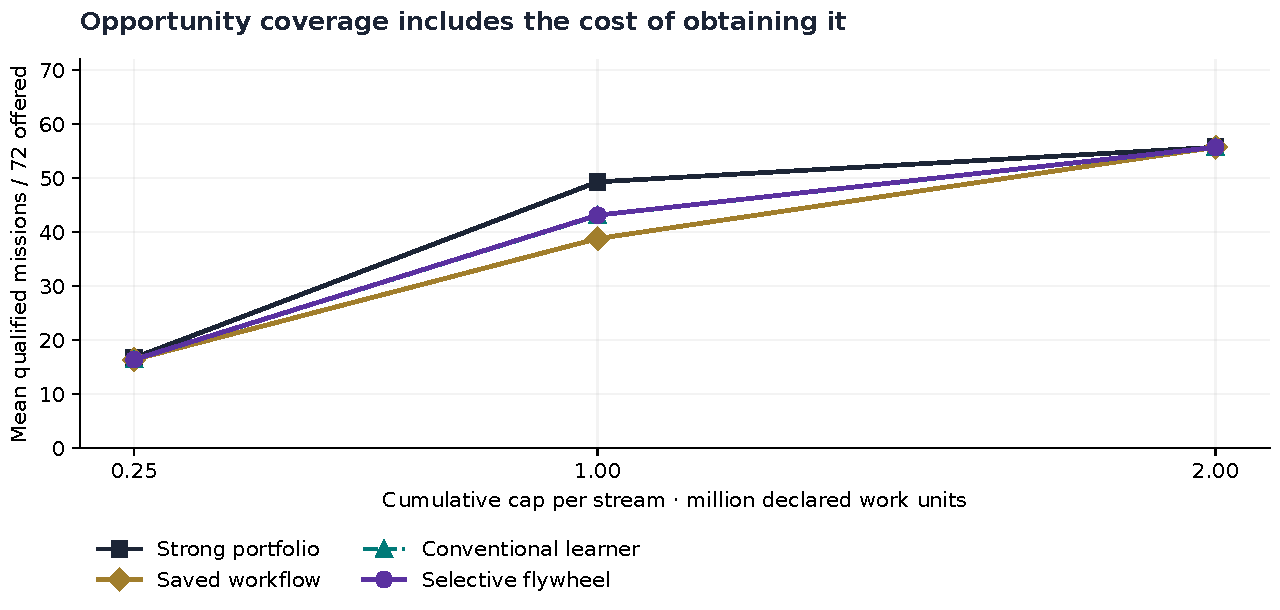
\includegraphics[width=\linewidth]{figures/opportunity-coverage.pdf}
\caption{Qualified coverage across the three registered cumulative caps. These are paired executions on the same offered tasks, not three independent task samples. Acquisition and operating history remain inside the charged budget; stopped missions remain in the denominator.}
\end{figure}

\begin{figure}[ht]\centering
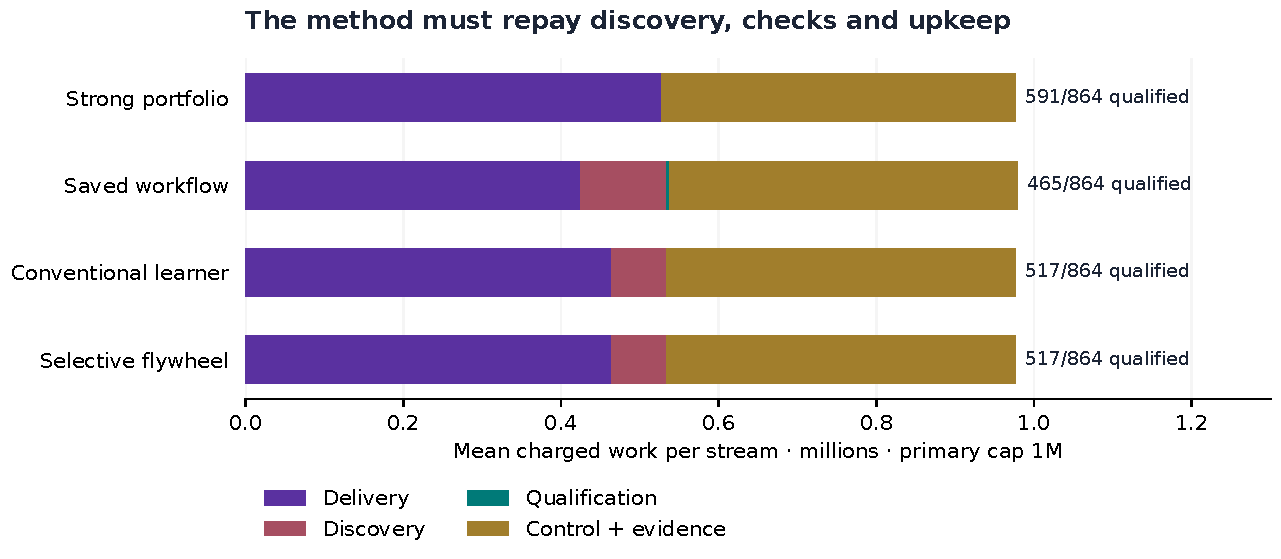
\includegraphics[width=\linewidth]{figures/full-cost-comparison.pdf}
\caption{Primary mean charged work, including delivery, discovery, qualification, control and evidence. The strongest portfolio's larger qualified output prevents a cheaper incomplete search from being called a productive inheritance advantage.}
\end{figure}

\subsection{Constructive succession under its separate research allowance}

All 12 inherited diagnostic streams construct three typed, correctness-qualified assets: dispatch, lookahead and repair. This is a structural lineage count, not a count of productive three-generation executions. The selected dispatch is critical-path-first in nine streams and shortest-duration-first in three. Lookahead settings vary across six retained recipes; repair selects quality, selective or stability-oriented modes. Experience therefore determines executable policy bytes within the authored language, rather than merely renaming a fixed answer.

The diagnostic records 2,411 inherited dispatch rollouts across all research and mission phases. All 12 fresh lookahead missions actually invoke their dispatch parent, and three qualify. Repair requires a sharper distinction: its 86 aggregate parent calls comprise 23 during training of eventual winners, 44 in losing-candidate training, 18 during selected-candidate qualification and only one on fresh mission work. Four qualification outputs both invoke the parent and qualify. No fresh repair does both. Ten retained stable repairs ignore that parent at delivery, and the selective repair takes its stable branch. Parent references alone therefore cannot support a claim of useful deep succession. The four mission positions across 12 streams yield 48 valid plans and 36 deadline-qualified deliveries: 12/12 founders and 24/36 later missions. Every one of the 36 retained assets is labeled \artifact{DIAGNOSTIC_CORRECTNESS_ONLY}; none passes the registered full-investment forecast in that inherited treatment.

\begin{table}[ht]\centering\small
\begin{tabularx}{\linewidth}{Yrrrr}
\toprule
Ancestry treatment & Valid / 48 & Qualified / 48 & Mean work & Lineages / 12 \\
\midrule
Inherited & 48 & 36 & 888,009.5 & 12 \\
Removed & 48 & \textbf{37} & \textbf{225,339.3} & 0 \\
Rebuilt & 48 & 36 & 2,239,765.9 & 12 \\
Equivalent replacement & 48 & 36 & 889,359.1 & 12 \\
\bottomrule
\end{tabularx}
\caption{Separate 5,000,000-unit diagnostic ceiling; all four missions include the founder. Rebuilding and equivalent replacement preserve every fresh schedule in all 12 paired streams. Removing ancestry prevents the authored child construction while leaving the conventional planner available.}
\end{table}

Rebuilding recovers the exact ancestral content on all 36 reconstruction events. Inheritance uses \textbf{60.35\% less work} than rebuilding. Equivalent normalized replacements preserve every fresh schedule, supporting equivalence of the substituted method behavior rather than dependence on a label. These interventions demonstrate conditional reconstruction savings; they do not by themselves prove that every retained child needs its recorded parent. The strongest executed succession claim is dispatch-to-lookahead on fresh work, plus parent use in repair construction/qualification. Parent-call counters are producer instrumentation; the independent audit attributes and reconciles them against exact raw records, while the separate checker verifies returned outputs. A call alone proves neither necessity nor value.

They do not support a net delivery advantage. Removing ancestry leaves no three-stage chain, yet the strong conventional fallback qualifies one more mission and costs substantially less. Eight of 12 removed-parent streams change at least one schedule. This preserves negative transfer and a cheaper alternative. In one descriptive fresh lookahead case, stream 10, inheritance reduces makespan from 50 to 47 while both versions qualify, at 16,214 versus 9,704 mission units; the complete 12-pair record also contains the losses. This isolated quality gain does not establish full-investment payback or survival against every specialist. The diagnostic demonstrates what a retained method can construct; it does not show that constructing it is the best way to satisfy the current finite demand.

\paragraph{An inspectable first lineage.}
The first stream supplies a concrete four-mission trace. The founder plan completes at slot 47. A learned critical-path rule then serves a different ordinary task at slot 39, meeting its independently checked lower bound. Its width-2, one-step lookahead child serves a tighter task at slot 36 but misses its deadline. A quality-oriented repair child preserves locked work and finishes at slot 51, with displacement 14, also missing its deadline. The latter misses remain in the record. The parent/child digests begin \artifact{7cebe063}, \artifact{7040e32c} and \artifact{0b17530e}; full ASTs, scopes, checks and lineage are in the first diagnostic checkpoint. This stream costs 869,191 units overall.


\begin{figure}[ht]\centering
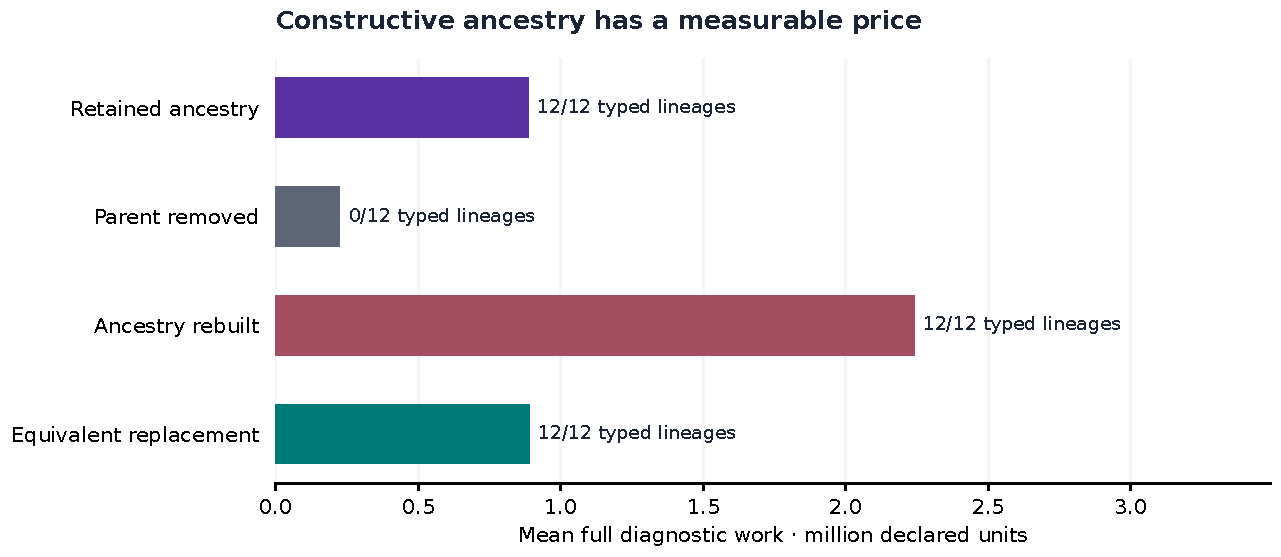
\includegraphics[width=\linewidth]{figures/ancestry-interventions.pdf}
\caption{The four ancestry interventions have distinct meanings. Removing a parent may block its child while leaving an effective conventional solver available. Rebuilding pays acquisition again; a semantically equivalent replacement tests dependence on useful behavior rather than the asset's label. Correctness-only diagnostic retention is separate from primary economic admission.}
\end{figure}

\subsection{The native specialist remains a serious alternative}

On the prespecified 36-task subset, the fixed interpreted portfolio produces 36 valid plans and meets 27 deadlines, at a measured mean preparation/check interval of 20.13\,ms. The native deadline model meets 31 deadlines. The solver reports four deadline models infeasible and reaches one solve limit without a qualifying result. Its mean native-and-check interval is 278.11\,ms; the practical workflow that also retains the known portfolio fallback averages 298.24\,ms and preserves 36 valid results.

The makespan model likewise qualifies 31/36 and returns 36 valid plans. It reports 29 optimal objective statuses and seven time-limited incumbents; the raw gap and dual-bound fields are preserved. Its mean end-to-end interval, including the independently checked portfolio upper bound, is 1,021.78\,ms. Shared native process startup adds 405.02\,ms to the campaign. These are measured physical intervals on one host, not conversions from the primary work tariff. A deadline mode's optimal status concerns its zero-objective feasibility model, not optimal makespan; returned feasible schedules are independently checked, while infeasibility and optimality statuses are solver reports without separately verified proof certificates.

The additional four qualified deadlines come from a strong established specialist. They are not improvements discovered by the flywheel. The reference illustrates a practical quality/latency choice that a future hybrid may exploit under a common, prospectively measured budget. The present experiment does not establish such a hybrid's overall superiority or price its extra computation as revenue.


\subsection{Counterexamples improve screening before they repay acquisition}

The separately frozen development probe executes the DOCX's challenge process. Three seeded defective creator artifacts produce substantiated objections, corrected outputs and retained regression cases. Two objections come from the bounded challenger; the locked-bound case is a review-specified counterexample. A fourth, deliberately false objection claims that overlapping jobs necessarily violate a pooled crew constraint. The adjudicator refutes it because concurrent demand equals available capacity. The correct result is retained.

The probe then compares seven prespecified candidate variants on 14 new diagnostic cases, with no protected confirmation inputs. Without early assets, the unchanged final checker uses 70 calls and 105,994 reference units. Screening the retained counterexamples first reduces these to 37 calls and 53,721 units. Acquisition and retention cost 41,785 units, while retrieval adds 27,177. The first batch therefore costs \textbf{122,683 units}, a \textbf{16,689-unit loss}. The conventional regression suite given the same assets produces exactly the same checks, costs and decisions.

All arms retain one valid candidate and reject six flawed variants. Final correctness does not improve. The useful change is \emph{earlier} exposure of particular defects; the valid candidate pays additional screening overhead. Repeating the identical batch would save 25,096 recurring units after retrieval, giving a modeled two-batch acquisition payback. That calculation assumes the same future defect mix and does not establish observed demand, a population effect or profit.

This probe's frozen tariff charges one reference unit per retained or retrieved byte, unlike the main study's 64-byte envelope/checkpoint blocks. Its payback boundary is conditional on that declared model. The two unit systems are not added together or treated as physical CPU costs.

\begin{figure}[ht]\centering
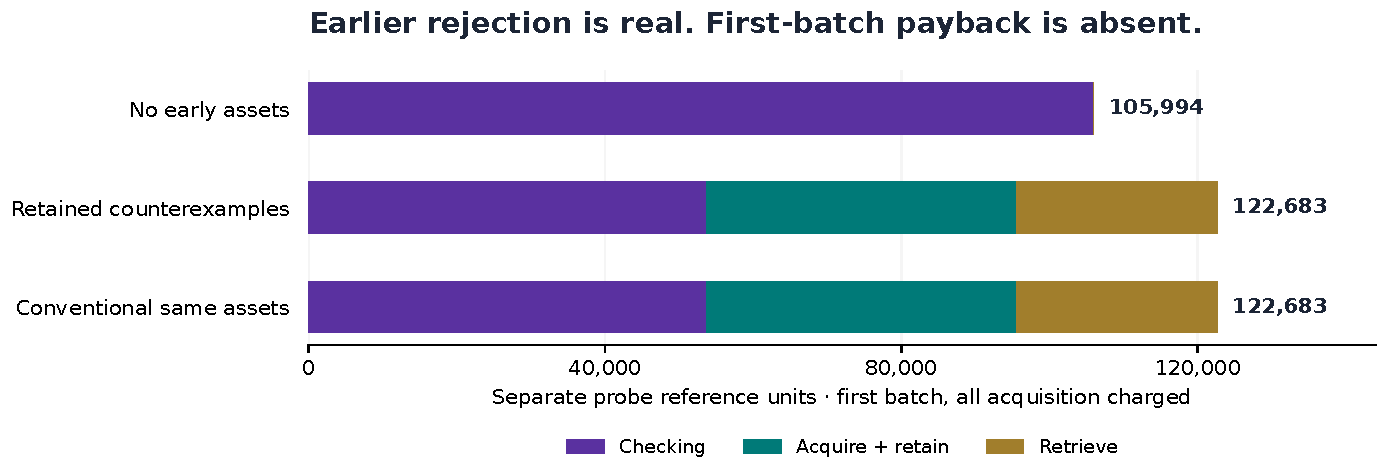
\includegraphics[width=\linewidth]{figures/regression-costs.pdf}
\caption{A verified counterexample is an asset with a carrying cost. Earlier rejection cuts checking work, but acquisition and retrieval reverse the first-batch saving. The conventional asset control is exactly equal. These are the separate development probe's reference units, not pooled main-study work units.}\label{fig:regression-costs}
\end{figure}

The raw challenge evidence, independent adjudications, revisions, regression assets, prospective probe protocol and frozen source identities are included under \artifact{review/}. The probe's seven deliberately seeded variants are not a random sample of production defects; no statistical population claim is made. Evaluator source and the final acceptance predicate remain unchanged throughout.

